\begin{center}
\textbf{Question:} What is the percentage increase from the March dividend\\
to the newly declared dividend?\par\smallskip
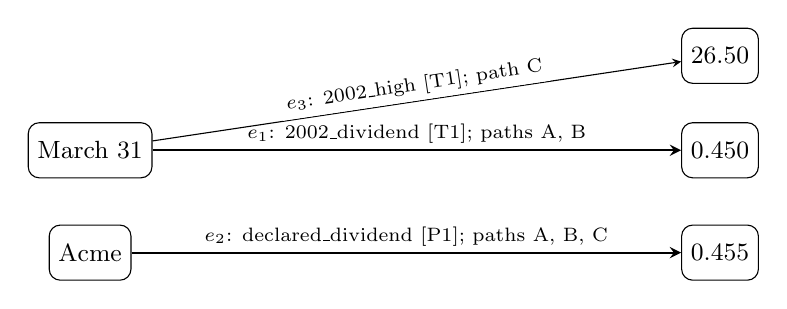
\begin{tikzpicture}[>=stealth,
 n/.style={draw,rounded corners,minimum height=7mm,font=\small},
 lab/.style={font=\scriptsize,fill=white,inner sep=2pt,align=center}]
\node[n] (row) at (0,0) {March 31};
\node[n] (old) at (8,0) {0.450};
\node[n] (high) at (8,1.2) {26.50};
\node[n] (company) at (0,-1.3) {Acme};
\node[n] (new) at (8,-1.3) {0.455};
\draw[->,thick] (row) -- node[lab,above] {$e_1$: 2002\_dividend [T1]; paths A, B} (old);
\draw[->] (row) -- node[lab,above,sloped] {$e_3$: 2002\_high [T1]; path C} (high);
\draw[->,thick] (company) -- node[lab,above] {$e_2$: declared\_dividend [P1]; paths A, B, C} (new);
\end{tikzpicture}\par
{\scriptsize Solid arrows: KG edges. T1: table source; P1: text source.
All values belong to the same illustrative report context.}\par\medskip
\end{center}
\noindent
\begin{minipage}[t]{0.315\linewidth}
\centering\small\textbf{Path A: correct operands}\\
\scriptsize Read $e_1$, read $e_2$;\\compute $(new-old)/old$.\par
\begin{lstlisting}[basicstyle=\ttfamily\scriptsize]
a = kg.get_neighbors(
 "March 31",
 "2002_dividend")[0]
b = kg.get_neighbors(
 "Acme",
 "declared_dividend")[0]
a, b = float(a), float(b)
result = (b-a)/a*100
\end{lstlisting}
\scriptsize Output: $+1.111\ldots\%$\\
Evidence: $\{e_1,e_2\}$\\
Execution: success\\
Score: $7.25$
\end{minipage}\hfill
\begin{minipage}[t]{0.315\linewidth}
\centering\small\textbf{Path B: wrong operation}\\
\scriptsize Read $e_1$, read $e_2$;\\reverse subtraction.\par
\begin{lstlisting}[basicstyle=\ttfamily\scriptsize]
a = kg.get_neighbors(
 "March 31",
 "2002_dividend")[0]
b = kg.get_neighbors(
 "Acme",
 "declared_dividend")[0]
a, b = float(a), float(b)
result = (a-b)/a*100
\end{lstlisting}
\scriptsize Output: $-1.111\ldots\%$\\
Evidence: $\{e_1,e_2\}$\\
Execution: success\\
Score: $7.25$
\end{minipage}\hfill
\begin{minipage}[t]{0.315\linewidth}
\centering\small\textbf{Path C: wrong operand}\\
\scriptsize Read $e_3$, read $e_2$;\\use price as old dividend.\par
\begin{lstlisting}[basicstyle=\ttfamily\scriptsize]
a = kg.get_neighbors(
 "March 31",
 "2002_high")[0]
b = kg.get_neighbors(
 "Acme",
 "declared_dividend")[0]
a, b = float(a), float(b)
result = (b-a)/a*100
\end{lstlisting}
\scriptsize Output: $-98.283\ldots\%$\\
Evidence: $\{e_3,e_2\}$\\
Execution: success\\
Score: $7.25$
\end{minipage}
\begin{center}
\small\textbf{Execution success + accessed evidence do not guarantee correctness.}
\end{center}
